\chapter{Graph Denoising}
In the following chapter, the connection between graphs and the domain of denoising in high-noise 
domains, such as cryo-EM, is established.
First, a broad definition of graphs is given and further, the term "Graph Denoising" is
introduced and explained. Finally, the connection to Graph Laplacian is established
and different opportunities exploiting for a good denoising algorithms are shown.


\section{Graph Foundations}
Graphs are a powerful representation of data, simple but with high expressiveness. 
Real world data could be in graph structure already, like social networks, citation networks,
protein interaction networks or google search. 
If not already in graph structure, a graph can be artificially constructed with methods like k-nearest neighbours (k-NN) or others.

\paragraph{Graph Learning:} is a popular research area and got a lot of attention in recent years.
It is a way of applying Machine Learning (ML) on graphs and algorithms emerged from ML but also other fields.
When a graph is available, one can start using Graph Learning algorithms for solving tasks.
Popular tasks are node classification or link prediction within a graph. One tries to learn from node and edge features 
as well as the topology of the graph and tries to map information to a model, which allows prediction or classification.
Another popular task in Graph Learning is community detection, where the aim is to identify cluster of nodes within the input graph.
Further, graphs are highly popular for dimensionality-reduction, where 
graph algorithms provide a helpful tool, as ordinary algorithms like principle component analysis fail.

\subsection{Graph definition}
A graph is defined as  $G = \langle V,E \rangle$, where $V$ is a set of 
vertices (or nodes) and $E$ is a set of edges (or links). 
Edges are defined as a set of tuples $(i, j)$, where $i$ and $j$ determine the index of the vertices in the graph.

\paragraph{Graph properties:}
A graph can be either \textit{directed} or \textit{undirected}. 
In a directed one, a edge points explicitly from one node to another, which means that edge $(i, j) \neq (j, i)$. 
In undirected graphs the ordering does not matter and  $(i, j) = (j, i)$.

The \textit{neighbourhood} of a node $\mathcal{N(i)} = \forall x $ is defined as all adjacent nodes 
of $i$, or in other words, there is an edge between the nodes. 
Further, edges can have \textit{weights}, which is a method to define importance to neighbours of a node.
If edges are dealing with weights, the term \textit{weighted} graph is used.
The \textit{degree} of a node are the number of incoming edges.

\paragraph{Adjacency matrix:}
To do calculations with graphs, it is common to translate graphs in a well suitable mathematically
form, which are matrices.
The adjacency matrix can be seen as a way of representing graphs as a matrix.
The (binary) adjacency matrix of graph $G$ is defined as follows:
\begin{equation}
    \label{eg:AdjacencyMatrix}
    A_{ij} =    
    \begin{cases}
        %1  & \text{if } \norm{\biggl y_i - y_j \biggr} < \tau\\
        1  & \text{if } (i, j) \in E \\
        0, & \text{otherwise}
    \end{cases}
\end{equation}

The matrix $A$ has dimension $\mathbb{R}^{N \times N}$ and the indices of the matrix correspond to the nodes of the graph.
If there is an edge between two nodes, the entry in the matrix will be set to $1$, otherwise to $0$.
This leads to an unweighted graph, as the weight of all edges will be $1$, but could easily be extended by assigned not just values of $1$ or $0$. 

When the graph is undirected, the resulting matrix will be symmetric. 
Eigenvalues of $A$ are also called \textit{spectrum} of the graph.


\subsection{Graph Construction}
3) General framework for constructing a graph:
a) Each vertex is associated to some feature/signal/whatever $x\in \mathcal{X}$, for some space arbitrary space $\mathcal{X}$.
b) We construct the graph $G_0$ using: $d(x_i,x_j) < \tau$, $\tau$ is a threshold, or k-NN (defined it here in one line).
c) For simplification, and because it covers already most cases, we will work on $\mathcal{x}= R^M$
d) There are some applications, as we will see (or have seen if already introduced), where we have only access to a noisy version of the true signal:
 $y = x + \eta$, where $y,x \in R^N$, and eta i.i.d follow Gaussian $(0,sigma^2)$.
e) Then we defined the noisy graph G as in b)

\label{sec:graphConstruction}
When data is not available as a graph, it can be constructed from the data.
Consider data from space $\Omega = \mathbb{R}^M $, but could basically be any arbitrary space.
Then, each node is associated with some element $x \in \mathcal{\Omega}$.
Further, the graph $G$ can be constructed by using:

\begin{equation}
    \label{eq:graphConstruction}
    A_{ij} =    
    \begin{cases}
        1  & \text{if } d(x_i, x_j) < \tau\\
        0, & \text{otherwise}
    \end{cases}
\end{equation}

where $n_i$, $n_j$ are nodes from indices $i,j$, $d$ is a similarity measure between two nodes and $\tau$ is a threshold, 
when to consider two nodes to be adjacent. K-NN is one possible implementation, where for every node, $k$ neighbours will be defined
The neighbourhood of node $i$ is defined as $\mathcal{N}_i$ and consists of the nodes, with the $k$ smallest similarity measure.

\paragraph{Noise regime}
In the case of high noise regime, observation of $x$ it not possible.
Measurements will give access to  $y = x + \eta$ where $y,x \in \Omega$ and the noise $\eta$ drawn from gaussian distribution $\mathcal{N} \sim (0,\sigma^2)$.
The \textit{noisy graph} $G_0$ can be constructed as in equation~\ref{eq:graphConstruction}, but replacing $y$ with $x$:
\begin{equation}
    \label{eq:graphConstructionNoise}
    A_{ij} =    
    \begin{cases}
        1  & \text{if } d(y_i, y_j) < \tau\\
        0, & \text{otherwise}
    \end{cases}
\end{equation}


\section{Graph Denoising definition}

First of all, Graph Denoising is not a common term in literature, but it is rather related to signal or image denoising.
Reconstruction of a true signal given noisy observation signal is done via averaging, that can be performed
locally, by the calculus of variations or in the frequency domain\cite{noneLocalMean}. 

In the last section, noisy graph $G_0$ was introduced and the aim is to denoise this graph,
which basically means to estimate the original graph $G$ from a given noisy graph $G_0$.

\begin{tcolorbox}[colback=red!5!white,colframe=red!75!black]
    The goal of the Master Thesis is to introduce a method to estimate 
    the original graph $G$ based on an observed noisy graph $G_0$.
\end{tcolorbox}

\paragraph{Noisy Graph:}
For every noisy graph, there exists an original graph $G = \langle V,E \rangle$.

The noisy graph can be further defined as follows:
\begin{equation}
    \begin{aligned}
        G_{noisy} &= \langle V,E_{noisy} \rangle,  \\ 
        \text{ with }  E_{noisy} &= E \setminus  E^{-} \cup  E^{+}, \\ 
         E^{-} & \subseteq E, \\
         E^{+} \cap E &= \emptyset
    \end{aligned}
\end{equation}

The noisy graph consists of the same nodes as the original graph. From
the original graphs edges, some are removed (denoted by $E^{-}$) and some are added
(denoted by $E^{+}$).

The adjacency matrix of $G_{noisy}$ is denoted by $\bar{A}_{ij}$.
The task of Graph Denoising, can therefore be written as:
\begin{equation}
    \bar{A} \xrightarrow[method]{Graph-denoising} \tilde{A} \approx A
\end{equation}

Where $\bar{A}$, $\tilde{A}$, $A$ denotes the adjacency matrix from noisy input graph, denoised
 graph and original graph respectively.

\subparagraph{Connection to link prediction}
Link prediction is a task in Graph Learning. 
The idea is to predict existence of a link (edge) between two nodes.
The task can be formulated as a missing value estimation task. A model $M_p$ is learned
from a given set of observed edges. The model finally maps links to probabilities
$M_p : E^{\prime} \rightarrow [0,1]$ where $E^{\prime}$ is the set of potential links.

We define $U$ as the set of all possible vertices of $G$, therefore $E \subseteq U$.
Obviously, graph denoising can be seen as a link prediction problem.

The difference is, that in link prediction a model from a set of observed links is learned
$E_{observed} \subseteq E$ and in Graph Denoising the model is learned from 
$E_{observed} \subseteq U$. 

\subsection{Non local means:}
Non local means is a state-of-the-art image denoising method \cite{noneLocalMean}.
For a given noisy image $v$, the denoised image is defined as $NL[v](i) = \sum{w(i,j) \; v(j)}$.
where $w(i,j)$ is the weight between pixel $i$ and $j$. The weight can be seen as a similarity measure of the two pixels.
Moreover, these similarities are calculated over square neighbourhoods of  two pixels,
where the $\ell2$-norm of the neighbourhood is used.
Similar pixel neighbourhoods have a large weight and different neighbourhoods have a small weight.
More general, the denoised image pixel $i$ is computed as an weighted average of all pixels in the 
image, therefore, in a non local way.


\section{Graph Laplacian}
The Graph Laplacian is a matrix that represents the graph and can be used to find many important properties of the graph, 
a good overview can be found by \cite{tutorialSpectralClustering, SpectralGraphTheory}. 
It is defined as follows:
\begin{equation}
    L = D - A,
\end{equation}

where $A$ is the adjacency matrix and $D$ the degree matrix (diagonal matrix with degree of nodes as entries).

\paragraph{Manifolds:}
\label{sec:manifolds}

In high-dimensional data euclidean distances are not meaningful in the sense that they will not capture similar data well.
Graph Laplacian can be used to compute a \textit{Manifold}, which can help in such a scenario. In the manifold space, euclidean distances make sense again. 
Let the manifold $M$ be defined as $\mathcal{M} = \{ f(x), f \in C^K, f: \mathbb{R}^D \to \mathbb{R}^d \}$.
Manifolds are a well established mathematical concept. In the Master Thesis, we will only consider 
$C^k$ differentiable d-dimensional manifold defined by $\mathcal{M}$. 
When $d \ll D$, the manifold defines a \textit{low dimensional embedding}, which maps from a high dimensional space 
$\mathbb{R}^D$ to a low dimensional space $\mathbb{R}^d$.

Lets give two popular examples of such manifolds, namely the \textit{circle} and the \textit{sphere}.
The circle is a 1D manifold, where $d=1$ and $D=2$. A sphere is a 2D manifold, with $d=2$ and $D=3$.

\subparagraph{Manifold assumption:}
\label{sec:manifoldAssumption}
The manifold assumption is a popular assumption for high-dimensional datasets.
For a given dataset in high-dimension, one can assume that data points are samples drawn from a low-dimensional manifold,
that embeds the high-dimensional space. Therefore, if the underlying manifold can be approximated, a dimensionality reduction
is established as one can embed the data points in the low-dimensional manifold space.
There is a complete area of research devoted to this manifold assumption called Manifold Learning\cite{ManifoldLearning}.

\begin{tcolorbox}[colback=red!5!white,colframe=red!75!black]
    In the field of classical tomography and cryo-EM, the manifold is well defined for none-noisy data.
    In the 2D case of classical tomography, the underlying manifold is a circle, whereas in 3D case of cryo-EM the manifold
    if defined as a sphere.
    This fact can be exploited during learning, by using the wasserstein loss function (see \ref{sec:wasserstein-metric}).
\end{tcolorbox}

The manifold, and therefore, a low-dimensional embedding, can be calculated the following:

\begin{enumerate}
    \item Construct the knn-graph from our observations (see section~\ref{sec:graphConstruction}).
    \item Calculate the (normalized) Graph Laplacian.
    \item Extract the second, third (and fourth) smallest eigenvectors.
\end{enumerate}

\begin{figure}[H]
    \centering
    \subbottom[Shepp-Logan phantom          \label{fig:phantom}]{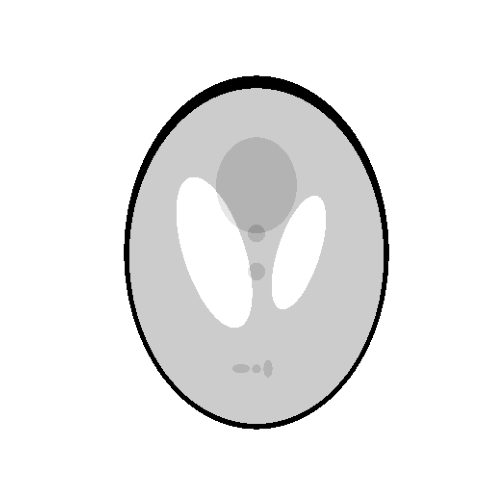
\includegraphics[width=0.18\textwidth]{phantom.png}}
    \subbottom[Original sinogram            \label{fig:ps:phantom_sinogram}]{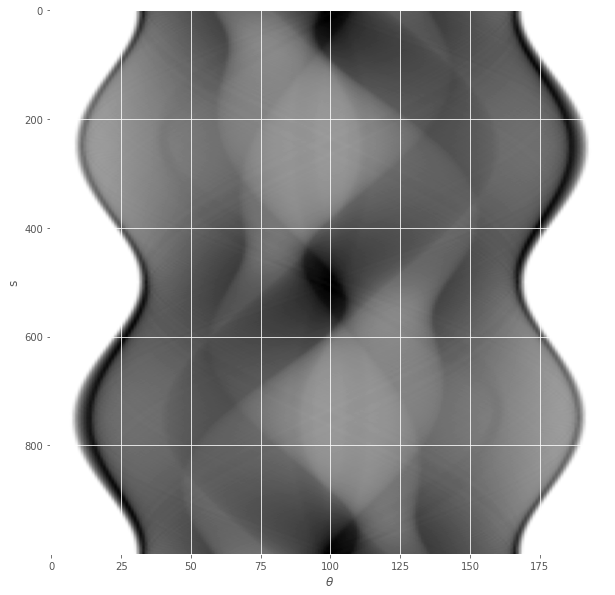
\includegraphics[width=0.18\textwidth]{phantom_sinogram.png}}
    \subbottom[Noisy sinogram               \label{fig:phantom_sinogram_noisy}]{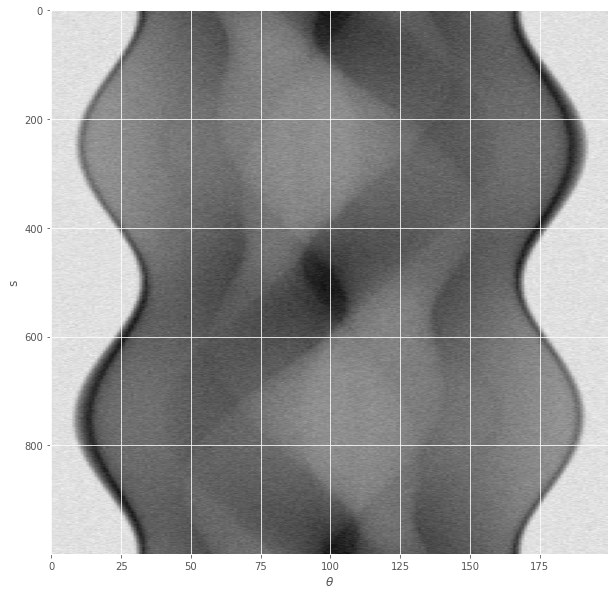
\includegraphics[width=0.18\textwidth]{phantom_sinogram_noisy.png}}
    \subbottom[2nd and 3rd smallest eigenvector of Graph Laplacian      \label{fig:phantom_second_third_evec}]{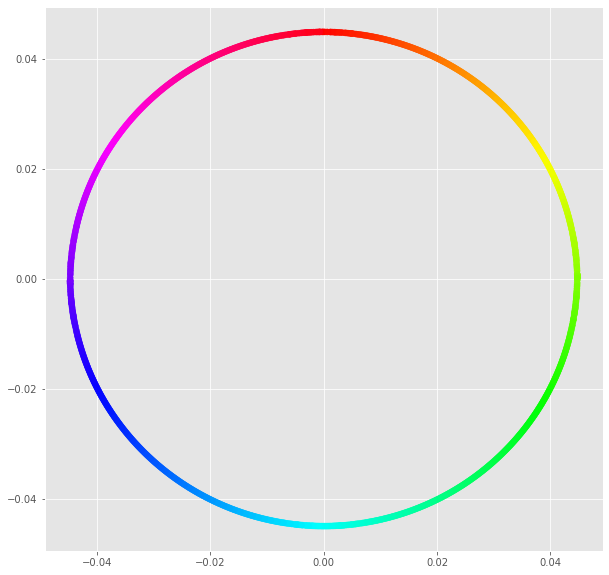
\includegraphics[width=0.18\textwidth]{phantom_second_third_evec.png}}
    \subbottom[2nd and 3rd smallest eigenvector of noisy Graph Laplacian\label{fig:phantom_second_third_evec_noisy}]{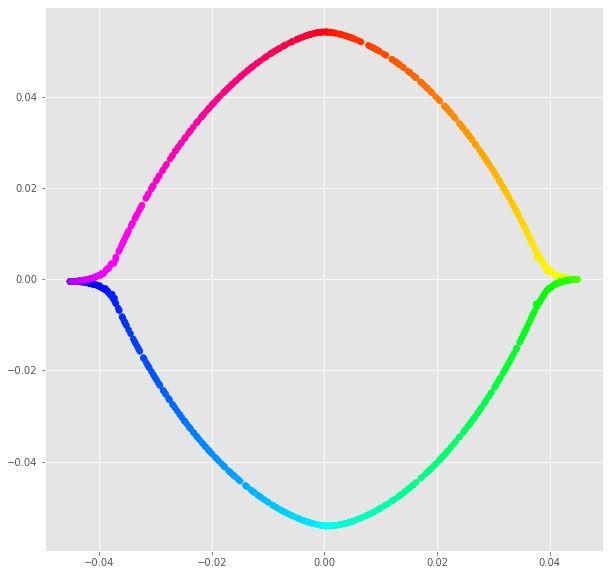
\includegraphics[width=0.18\textwidth]{phantom_second_third_evec_noisy.png}}
    \caption{Shepp-Logan phantom manifold}
\end{figure}

In Figure~\ref{fig:phantom_second_third_evec} the manifold calculated from the original Graph Laplacian
can be seen and it is a perfect circle. Next to it, in Figure~\ref{fig:phantom_second_third_evec_noisy}
the noisy version with $\sigma=2$ is plotted and the manifold is circle like but not at all like from the original one.

The more noise we add, the less the manifold looks like a circle. In Figure~\ref{fig:phantom_second_third_evec_noisy_high}
the manifold for $\sigma=100$ is plotted.

\begin{figure}[H]
    \centering
    \subtop[Highly noisy sinogram               \label{fig:phantom_sinogram_noisy_high}]{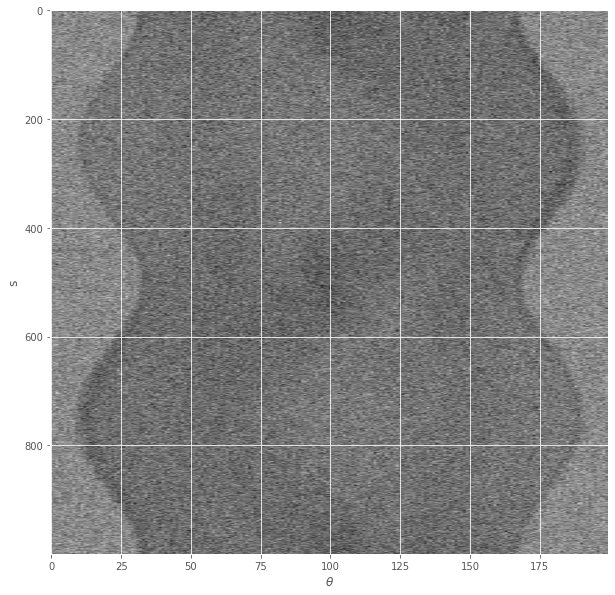
\includegraphics[width=0.4\textwidth]{phantom_sinogram_noisy_high.png}}
    \subtop[2nd and 3rd smallest eigenvector of Graph Laplacian      \label{fig:phantom_second_third_evec_noisy_high}]{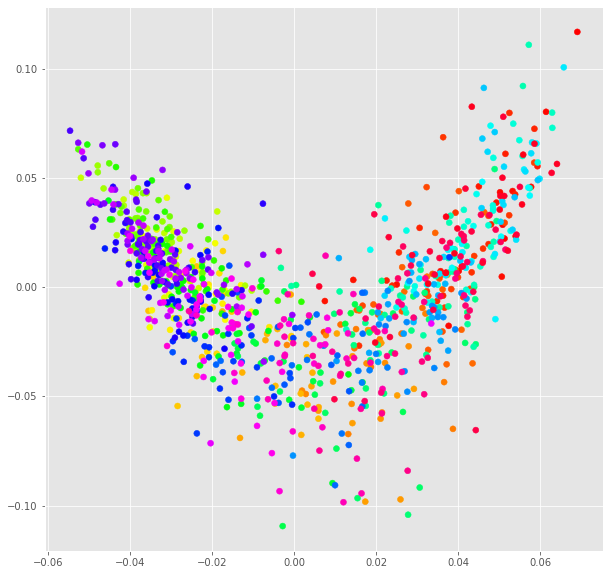
\includegraphics[width=0.4\textwidth]{phantom_second_third_evec_noisy_high.png}}
    \caption{Shepp-Logan phantom manifold for high noise level}
\end{figure}

In all the plots, knn-graph have been constructed with $k=10$. 

\textbf{TODO: If time, define SNR properly and do some other plots with SNR smaller to 1}

\subsection{Connection to machine learning}

Graph Laplacian is used for dimensionality reduction for high-dimensional data, as well as spectral clustering and semi-supervised learning.
\citet{LaplaceRandomProjections} used Graph Laplacian in a complete other domain, namely in tomography. 
They showed that Graph Laplacian approximates the Laplace-Beltrami operator.
Further, Graph Laplacian is depended on the adjacency matrix $A$. 
If $A$ is noisy, Graph Laplacian will be noisy as well.


\begin{tcolorbox}[colback=red!5!white,colframe=red!75!black]
    In the Master Thesis, new experience of Graph Laplacian in the domain of tomography and denoising
    should be gained. Further, the connection with machine learning will be explored, hopefully allowing to learn a denoised 
    adjacency matrix to fully enable the power of Graph Laplacian.
\end{tcolorbox}


\subsection{Graph Deep Learning}
As already mentioned, Graph Denoising can be seen as a way of link predication. 
The state-of-the-art method for solving link prediction are graph deep learning approaches.
Graph deep learning is a fast evolving field in research. With Graph Neural Networks (GNN)\cite{GNN} the framework
for GNN has been established. 

Using Graph Convolutional Networks (GCN) \cite{GCN} for graph feature extraction is a popular way. 
Basically, with GCN a new feature representation is iteratively learned for the node features (edges features are not taken into account).
It can be seen as an averaging of nodes over their neighbourhood where all the neighbours get the same weight combined with some non-linear activation. 
To consider the node itself in the averaging process they apply to so-called "Renormalization trick", where self-loops are added to the 
adjacency matrix and after every layer, a normalization step is applied.The topology of the graph will not be adjusted during the learning process.

\citet{GAT} extended the concept of GCN with attention and not all the neighbouring nodes get the same weight (attention).
Simple Graph Convolutional Network (SGC) \cite{simpleGCN} proposed a simplified version of GCN.
They could verify their hypothesis that GCN is dominated by the local averaging step and the non-linear 
activation function between layers do not contribute to much to the success of GCN. 
Therefore, it can be seen as a way of power iteration (see \ref{sec:powerIterations} for further information) over the adjacency matrix with normalization in every layer.
\citet{dynamicGCN} proposed a extended version of GCN by not operating on the same graph in every layer but adopting
the underlying graph topology layer by layer.

\begin{tcolorbox}[colback=red!5!white,colframe=red!75!black]
    In the Master Thesis, the connection between Graph Laplacian and GNNs should be further exploited.
    The fact, that \cite{simpleGCN} could simplify the existing GCN algorithm is motivation enough,
    that similar connections can be drawn in other fields of Graph Learning.
\end{tcolorbox}

